\documentclass[preprint,authoryear,12pt]{elsarticle}

\usepackage{graphicx}
\usepackage{booktabs}
\usepackage{adjustbox}
\usepackage{amsmath}
\usepackage{siunitx}
\usepackage[hypertexnames=false]{hyperref}
\usepackage{float}
\usepackage{placeins}
\usepackage[margin=1in]{geometry}

\graphicspath{{out/figures/}}
\newcommand{\AirImproveMax}{0.30}
\newcommand{\AirImproveMin}{0.20}
\newcommand{\AirPPDImproveMax}{7.2}
\newcommand{\AirPPDImproveMin}{5.7}
\newcommand{\AllAirControlWins}{6}
\newcommand{\LargerAirImprove}{0.20}
\newcommand{\LargerAirPPDImprove}{7.0}
\newcommand{\LargerDeltaTaMax}{5.91}
\newcommand{\LargerDeltaTaMin}{4.56}
\newcommand{\LargerOneStepLoad}{32.1}
\newcommand{\LargerRadImprove}{0.15}
\newcommand{\LargerRadPPDImprove}{5.4}
\newcommand{\LargerStepPPD}{31.4}
\newcommand{\OlderAirImprove}{0.25}
\newcommand{\OlderAirPPDImprove}{6.0}
\newcommand{\OlderDeltaTaMax}{4.59}
\newcommand{\OlderDeltaTaMin}{3.54}
\newcommand{\OlderOneStepLoad}{20.1}
\newcommand{\OlderRadImprove}{0.19}
\newcommand{\OlderRadPPDImprove}{5.5}
\newcommand{\OlderStepPPD}{31.4}
\newcommand{\OneStepLoadMax}{32.1}
\newcommand{\OneStepLoadMin}{18.4}
\newcommand{\OneStepPPDMax}{50.6}
\newcommand{\OneStepPPDMin}{21.1}
\newcommand{\PPDAtHalf}{10.2}
\newcommand{\PPDAtOne}{26.1}
\newcommand{\ProfileCount}{4}
\newcommand{\RadImproveMax}{0.23}
\newcommand{\RadImproveMin}{0.15}
\newcommand{\RadPPDImproveMax}{6.9}
\newcommand{\RadPPDImproveMin}{5.3}
\newcommand{\RadiantExergyWins}{5}
\newcommand{\ReferenceAirImprove}{0.26}
\newcommand{\ReferenceAirPPDImprove}{5.7}
\newcommand{\ReferenceDeltaTaMax}{4.65}
\newcommand{\ReferenceDeltaTaMin}{3.53}
\newcommand{\ReferenceOneStepLoad}{24.4}
\newcommand{\ReferencePMVFactor}{0.0740}
\newcommand{\ReferenceRadImprove}{0.19}
\newcommand{\ReferenceRadPPDImprove}{5.3}
\newcommand{\ReferenceStepPPD}{31.4}
\newcommand{\ScenarioCount}{6}
\newcommand{\SmallerAirImprove}{0.30}
\newcommand{\SmallerAirPPDImprove}{7.2}
\newcommand{\SmallerDeltaTaMax}{3.91}
\newcommand{\SmallerDeltaTaMin}{2.98}
\newcommand{\SmallerOneStepLoad}{18.4}
\newcommand{\SmallerRadImprove}{0.23}
\newcommand{\SmallerRadPPDImprove}{6.9}
\newcommand{\SmallerStepPPD}{31.4}


\journal{Building and Environment}

\begin{document}

\begin{frontmatter}

\title{Predicted Mean Vote as a Weak Sole Control Signal: Pathway, Step-Response, and Exergy Limits of PMV-Based Thermal Control}

\author{Anonymous for review}

\begin{abstract}
Predicted Mean Vote (PMV) is widely used as both an indoor comfort index and a practical control target. This dual use is convenient, but it blurs several different meanings into a single scalar. This paper tests that ambiguity through a reproducible model-logic study built on an ISO 7730 implementation and two companion analyses: severe discomfort recovery with surrogate system exergy and profile-sensitive PMV step-response experiments. For a fixed occupant profile, PMV remains linear in thermal load, so a one-unit PMV step corresponds to a fixed load step of \SIrange{\OneStepLoadMin}{\OneStepLoadMax}{W/person} across the profiles tested. However, the environmental move needed to traverse one PMV label is not fixed. For the reference office profile, one-step recovery requires \SIrange{\ReferenceDeltaTaMin}{\ReferenceDeltaTaMax}{\celsius} of air-temperature change across the environmental families tested; for the larger and more highly clothed profile, the same one-step transition requires \SIrange{\LargerDeltaTaMin}{\LargerDeltaTaMax}{\celsius}. PPD restores some nonlinear acceptability meaning, but it does so only by remapping PMV: the same one-label PMV transition changes predicted dissatisfaction by \numrange{\OneStepPPDMin}{\OneStepPPDMax} percentage points across the tested transitions. Directed \SI{1}{\celsius} air shifts move PMV toward neutrality more strongly than directed \SI{1}{\celsius} radiant shifts in the current cases, and they also reduce PPD more strongly on average, but they do so mainly by changing convective heat loss, whereas radiant shifts act primarily through radiative exchange. In six severe discomfort archetypes, all-air control gives the shortest PMV recovery in \AllAirControlWins/\ScenarioCount\ cases, while radiant control minimizes estimated system exergy in \RadiantExergyWins/\ScenarioCount. These results indicate that PMV is useful as a bounded steady-state comfort index near neutrality, but physically underdetermined and physiologically incomplete as a sole control objective. PMV-only control collapses distinct pathway, acceptability, and system meanings into one scalar and should be paired with local discomfort and system-side metrics.
\end{abstract}

\begin{keyword}
thermal comfort \sep PMV \sep PPD \sep thermal control \sep radiant systems \sep exergy \sep pathway analysis
\end{keyword}

\end{frontmatter}

\section{Introduction}

Predicted Mean Vote (PMV) remains the default analytical language for steady-state thermal comfort in mechanically conditioned buildings \citep{Fanger1970,ISO7730_2025,ASHRAE55_2023}. It is compact, auditable, and deeply embedded in standards practice. That compactness is also the problem. In applied building work, PMV often shifts from a group-average comfort descriptor to something more ambitious: a variable to monitor, optimize, and control. Once treated that way, one scalar has to carry several meanings at once. It must stand in for thermal sensation, discomfort severity, pathway imbalance, and control effort. Those meanings are not equivalent.

This tension appears most clearly when PMV is used to reason about recovery. A one-unit PMV change from $-3$ to $-2$ is mathematically the same size as a change from $-1$ to $0$, but the practical meaning is not the same. One state is plainly severe discomfort, while the other is already near the usual comfort target of $|PMV| \le 0.5$. The same ambiguity holds for the environment and the system. If two control actions reach the same recovered PMV, they are often treated as equivalent recoveries even if one acts mainly through convection and the other through radiation, or if one demands substantially greater plant-side work.

The same problem appears one layer lower in the physics. Building practice often privileges air-temperature reasoning because it is measurable, actionable, and easy to connect to thermostat logic. That convenience is real, but it is not a complete description of occupant heat exchange. PMV inherits a similar convenience. It compresses convective, radiative, evaporative, and respiratory effects into one operationally legible index. The present paper argues that this convenience should be treated as conditional rather than complete.

The purpose of this paper is to separate those meanings rather than to reject PMV outright. The paper asks four bounded questions. First, what is the exact relationship between PMV and thermal load inside the implemented model? Second, what does the standard Predicted Percentage of Dissatisfied (PPD) mapping add, and what does it not add? Third, if equal PMV steps are taken as notional TSV-like transitions, do they imply equal environmental control moves? Fourth, if the same severe discomfort state is recovered by either air-side or radiant-side control, does the control ranking stay the same once approximate system exergy is introduced?

The paper answers these questions through a model-logic study rather than a validation study. It does not claim that PMV is physiologically complete, nor does it claim measured human-subject confirmation of the proposed pathway interpretation. Instead, it uses reproducible numerical experiments to show where PMV is exact, where it is underdetermined, and where it becomes a weak sole control target. The main argument is deliberately narrow: PMV/PPD remain useful near neutrality as bounded steady-state comfort indices, but they are inadequate as sole control objectives because equal PMV motion does not imply equal pathway meaning, equal physical intervention, or equal system cost.

\section{Methods}

\subsection{Model scope}

All calculations use the repository's existing ISO 7730 PMV implementation. The model is steady-state and whole-body. It resolves the thermal balance into convective, radiative, evaporative, and respiratory terms, then maps the resulting load to PMV and PPD. For a given occupant,
\begin{equation}
\mathrm{PMV} = \left(0.303 e^{-0.036 M} + 0.028\right)(H-L),
\end{equation}
where $M$ is metabolic rate in \si{W/m^2}, $H=M-W$ is internal sensible generation, and
\begin{equation}
L = Q_{\mathrm{conv}} + Q_{\mathrm{rad}} + E_{\mathrm{sk}} + Q_{\mathrm{res}}.
\end{equation}
PPD is then computed as
\begin{equation}
\mathrm{PPD} = 100 - 95 \exp\left(-0.03353\, \mathrm{PMV}^4 - 0.2179\, \mathrm{PMV}^2\right).
\end{equation}

The dry heat-transfer pathways are evaluated as
\begin{align}
Q_{\mathrm{rad}} &= 3.96 \times 10^{-8}\, f_{\mathrm{cl}} \left(T_{\mathrm{cl},K}^4 - T_{\mathrm{r},K}^4\right), \\
Q_{\mathrm{conv}} &= f_{\mathrm{cl}} h_c \left(T_{\mathrm{cl}} - T_a\right),
\end{align}
with clothing represented through the standard clothing-area factor $f_{\mathrm{cl}}$ and clothing insulation $I_{\mathrm{cl}}$ \citep{Fanger1970,ISO7730_2025}. This matters for interpretation. Clothing does not enter here as explicit geometry or exposed-skin fraction; the standard formulation treats its thermal effect through insulation and clothing area factor only.

The PMV formulation is therefore treated here as a set of conditional pathway closures inside a steady-state occupant heat balance rather than as a direct physiological measurement. The model therefore has clear scope boundaries. It does not represent dynamic thermoregulation such as vasoconstriction or shivering, it does not model local body segments, and it does not represent measured TSV data. It is used here to interrogate the internal logic of PMV/PPD and to compare pathway and control interpretations under that logic.

\subsection{Study structure}

The manuscript uses two companion studies.

The first, \textit{PMV balance relationship}, probes PMV algebra directly. It builds (i) a sampled PMV-versus-load dataset across many environmental states and metabolic levels, (ii) the deterministic PPD curve, (iii) zero-PMV contours in $(T_a, T_r)$ space under several humidity and air-speed conditions, (iv) profile-sensitive directed \SI{1}{\celsius} air and radiant perturbations, and (v) one-PMV-step air-response experiments across four environmental families. The PPD analysis is treated explicitly as an acceptability remapping layered on top of PMV rather than as independent physics.

The second, \textit{pathway discomfort}, constructs six severe discomfort archetypes for one representative office occupant and asks which single environmental lever recovers each state most directly. Recovery is judged first by normalized control displacement and then by a low-order system-side exergy surrogate.

The six severe archetypes are listed in Table~\ref{tab:scenarios}. They represent bulk cold, radiant cold, convective cold through draft, bulk hot, radiant hot, and hot humid still air. All were built to satisfy $|PMV| \geq 2$ in the baseline state for the representative office occupant before recovery.

\begin{table}[t]
\centering
\caption{Severe discomfort archetypes used for recovery and exergy comparisons.}
\label{tab:scenarios}
\begin{adjustbox}{max width=\textwidth}
\begin{tabular}{p{3.3cm}p{1.8cm}cccccc}
\toprule
Scenario & Class & $T_a$ & $T_r$ & RH & $v$ & PMV & PPD \\
\midrule
Severe cold bulk & bulk cold & 19.0 & 19.0 & 50 & 0.10 & -3.50 & 100.0 \\
Cold radiant sink & radiant cold & 23.0 & 17.0 & 50 & 0.10 & -2.90 & 98.6 \\
Cold high-airflow draft & convective cold & 20.0 & 20.0 & 50 & 0.60 & -4.74 & 100.0 \\
Severe hot bulk & bulk hot & 32.0 & 32.0 & 50 & 0.10 & 2.07 & 79.9 \\
Hot radiant gain & radiant hot & 29.0 & 35.0 & 50 & 0.10 & 2.05 & 79.1 \\
Hot humid still air & humid hot & 31.0 & 31.0 & 80 & 0.05 & 2.12 & 81.9 \\
\bottomrule
\end{tabular}
\end{adjustbox}
\begin{flushleft}\footnotesize All severe scenarios satisfy $|PMV| \geq 2$ for the representative office occupant before recovery.\end{flushleft}
\end{table}


\subsection{Occupant profiles}

The profile-sensitive PMV-step and directed \SI{1}{\celsius} experiments use four normative occupant archetypes rather than population distributions. This choice is deliberate. The paper is not trying to infer population prevalence; it is trying to show how profile assumptions change the relation among PMV, pathway watts, and control displacement. The four profiles vary age, sex, height, weight, clothing insulation, and metabolic rate. Body surface area is computed using the Du Bois relation \citep{DuBois1916}. Metabolic rate is expressed in both met and \si{W/person}.

\begin{table}[t]
\centering
\caption{Normative occupant profiles used in the profile-sensitive PMV step and 1$^\circ$C perturbation analyses.}
\label{tab:profiles}
\begin{adjustbox}{max width=\textwidth}
\begin{tabular}{p{3.1cm}cccccccc}
\toprule
Profile & Age & Sex & Height & Weight & BSA & Clo & Met & W/person \\
\midrule
Smaller female, lower-met & 30 & female & 160 & 55 & 1.56 & 0.45 & 0.8 & 72.7 \\
Reference office & 40 & male & 170 & 70 & 1.81 & 0.50 & 0.9 & 94.7 \\
Larger male, formal & 35 & male & 182 & 88 & 2.10 & 0.70 & 1.0 & 121.9 \\
Older layered occupant & 70 & female & 165 & 64 & 1.70 & 0.70 & 0.8 & 79.3 \\
\bottomrule
\end{tabular}
\end{adjustbox}
\begin{flushleft}\footnotesize Profiles are illustrative control-design archetypes. Age and sex are not explicit PMV inputs; they enter only through the assumed body size, clothing insulation, and metabolic rate.\end{flushleft}
\end{table}


The profiles are ``rock solid'' only in a bounded sense: they are explicit, reproducible, and literature-anchored as control-design archetypes. They are not demographic truth claims. Age and sex do not appear directly in the PMV equation; they enter only through the assumed values of body size, clothing insulation, and metabolic rate. This distinction is important because it limits what can be claimed about physiology from the current model.

This matters practically because the occupant baseline is not neutral. A control strategy built around a default office occupant already embeds a hidden normalization choice before any environmental control move is evaluated. In the present manuscript the reference office profile uses `0.9 met`, not `1.0 met`, specifically to avoid quietly inheriting a higher sedentary baseline. The resulting PMV slope and one-step thermal-load requirement are therefore profile-sensitive by construction rather than fixed properties of the environment alone.

\subsection{One-PMV-step and directed \SI{1}{\celsius} experiments}

Two separate perturbation families are used in the PMV-balance study.

The first is a directed \SI{1}{\celsius} response test. If a baseline state is colder than neutral ($PMV<0$), the model applies a warming move; if it is hotter than neutral ($PMV>0$), it applies a cooling move. This is done once by changing $T_a$ only and once by changing $T_r$ only. The resulting changes in PMV, PPD, total thermal load, and pathway watts are then recorded.

The second is a one-label PMV transition test. Starting states are solved such that PMV lies at approximately $-3$, $-2$, $-1$, $+1$, $+2$, or $+3$ under several environmental families. Air temperature is then solved again to move the profile one label toward neutrality: $-3 \rightarrow -2$, $-2 \rightarrow -1$, $-1 \rightarrow 0$, and the corresponding hot-side mirrors. This experiment isolates two subtle but important distinctions. Because PMV is linear in thermal load for fixed $M$, a one-unit PMV step implies a fixed load step within a given profile. It does not imply a fixed $\Delta T_a$. Because PPD is a nonlinear function of PMV, the same one-unit PMV step also does not imply a fixed change in dissatisfied fraction. Table~\ref{tab:stepsummary} keeps the evidence concrete by listing the neutral-still transitions for two representative profiles, while Figure~\ref{fig:stepresponse} shows the full family-to-family variation.

\begin{table}[t]
\centering
\caption{Representative one-label PMV transitions under the neutral-still family for two office profiles.}
\label{tab:stepsummary}
\begin{adjustbox}{max width=\textwidth}
\begin{tabular}{p{3.0cm}p{1.0cm}cccccc}
\toprule
Profile & Step & $\Delta T_a$ & $\Delta(H-L)$ & $\Delta PPD$ & $\Delta Q_{conv}$ & $\Delta Q_{rad}$ \\
\midrule
Reference office & -3$\rightarrow$-2 & 4.30 & 24.4 & 22.4 & -29.3 & 8.0 \\
Reference office & -2$\rightarrow$-1 & 4.57 & 24.4 & 50.6 & -28.6 & 7.8 \\
Reference office & -1$\rightarrow$0 & 4.57 & 24.4 & 21.1 & -28.1 & 7.7 \\
Reference office & +1$\rightarrow$0 & -4.57 & -24.4 & 21.1 & 28.2 & -7.8 \\
Reference office & +2$\rightarrow$+1 & -4.51 & -24.4 & 50.6 & 27.8 & -7.8 \\
Reference office & +3$\rightarrow$+2 & -4.43 & -24.4 & 22.4 & 27.3 & -7.7 \\
Larger male, formal & -3$\rightarrow$-2 & 5.42 & 32.1 & 22.4 & -42.5 & 14.4 \\
Larger male, formal & -2$\rightarrow$-1 & 5.74 & 32.1 & 50.6 & -41.5 & 14.2 \\
Larger male, formal & -1$\rightarrow$0 & 5.87 & 32.1 & 21.1 & -40.4 & 14.0 \\
Larger male, formal & +1$\rightarrow$0 & -5.72 & -32.1 & 21.1 & 40.7 & -14.3 \\
Larger male, formal & +2$\rightarrow$+1 & -5.75 & -32.1 & 50.6 & 39.7 & -14.0 \\
Larger male, formal & +3$\rightarrow$+2 & -5.62 & -32.1 & 22.4 & 38.8 & -13.9 \\
\bottomrule
\end{tabular}
\end{adjustbox}
\begin{flushleft}\footnotesize All rows are taken from the neutral-still environmental family to keep the evidence readable. The full family-to-family variation appears in Figure~\ref{fig:stepresponse}. Equal PMV steps retain the same body-load step within a profile, but not the same air-temperature move or dissatisfaction change.\end{flushleft}
\end{table}


\subsection{System-side exergy surrogates}

The severe-discomfort recovery study compares four single-lever controls: all-air sensible control, radiant-only control, airflow control, and latent control. To avoid treating $\Delta T_a$ and $\Delta T_r$ as if they had the same plant implication, the study adds low-order system-side surrogates:
\begin{align}
Q_{\mathrm{air}} &= \rho c_p \dot{V} |\Delta T_a|, \\
Q_{\mathrm{rad,sys}} &= h_r A |\Delta T_r|, \\
P_{\mathrm{fan}} &\propto v^3, \\
Q_{\mathrm{lat}} &= \dot{m} h_{fg} |\Delta W|.
\end{align}
These are converted to approximate electric / exergy input using fixed coefficient-of-performance assumptions. They are ranking devices, not full HVAC models.

\begin{table}[t]
\centering
\caption{System-side surrogate assumptions used to convert control moves into approximate exergy/electric input.}
\label{tab:system}
\begin{adjustbox}{max width=\textwidth}
\begin{tabular}{p{3.0cm}p{4.5cm}p{6.0cm}}
\toprule
Lever & Surrogate relation & Assumptions \\
\midrule
All-air sensible control & $Q = \rho c_p \dot V |\Delta T_a|$ & 0.05 m$^3$/s, COP = 3.0/3.0 \\
Radiant control & $Q = h_r A |\Delta T_r|$ & $h_r$ = 4.7 W/m$^2$K, $A$ = 12 m$^2$, COP = 4.5/5.5 \\
Airflow control & $P \propto v^3$ & fan power max = 60 W at 1.2 m/s \\
Latent control & $Q = \dot m h_{{fg}} |\Delta W|$ & $h_{fg}$ = 2.45e+06 J/kg, COP = 1.8/1.0 \\
\bottomrule
\end{tabular}
\end{adjustbox}
\begin{flushleft}\footnotesize These are low-order plant surrogates used only for ranking, not full HVAC models.\end{flushleft}
\end{table}


\section{Results}

\subsection{PMV is linear in thermal load, and PPD adds acceptability curvature but not new physics}

Figure~\ref{fig:foundations} shows the algebraic core of the argument. For a fixed metabolic rate, PMV lies on a straight line with thermal load. In the current implementation, the PMV factor for the reference office condition is \ReferencePMVFactor. This means PMV is not a free-floating vote regressor inside the model; it is a scaled thermal-load expression. The PPD curve adds nonlinearity only by remapping PMV to a dissatisfied fraction. It does not recover lost pathway meaning or physiological detail. It also imposes a minimum of \SI{5}{\percent} dissatisfied even at PMV = 0, rises to about \SI{\PPDAtHalf}{\percent} at $|PMV| = 0.5$, and reaches about \SI{\PPDAtOne}{\percent} at $|PMV| = 1.0$. PPD therefore restores some operational meaning near the comfort rim, but it does not add a new physical or physiological model.

\begin{figure}[H]
\centering
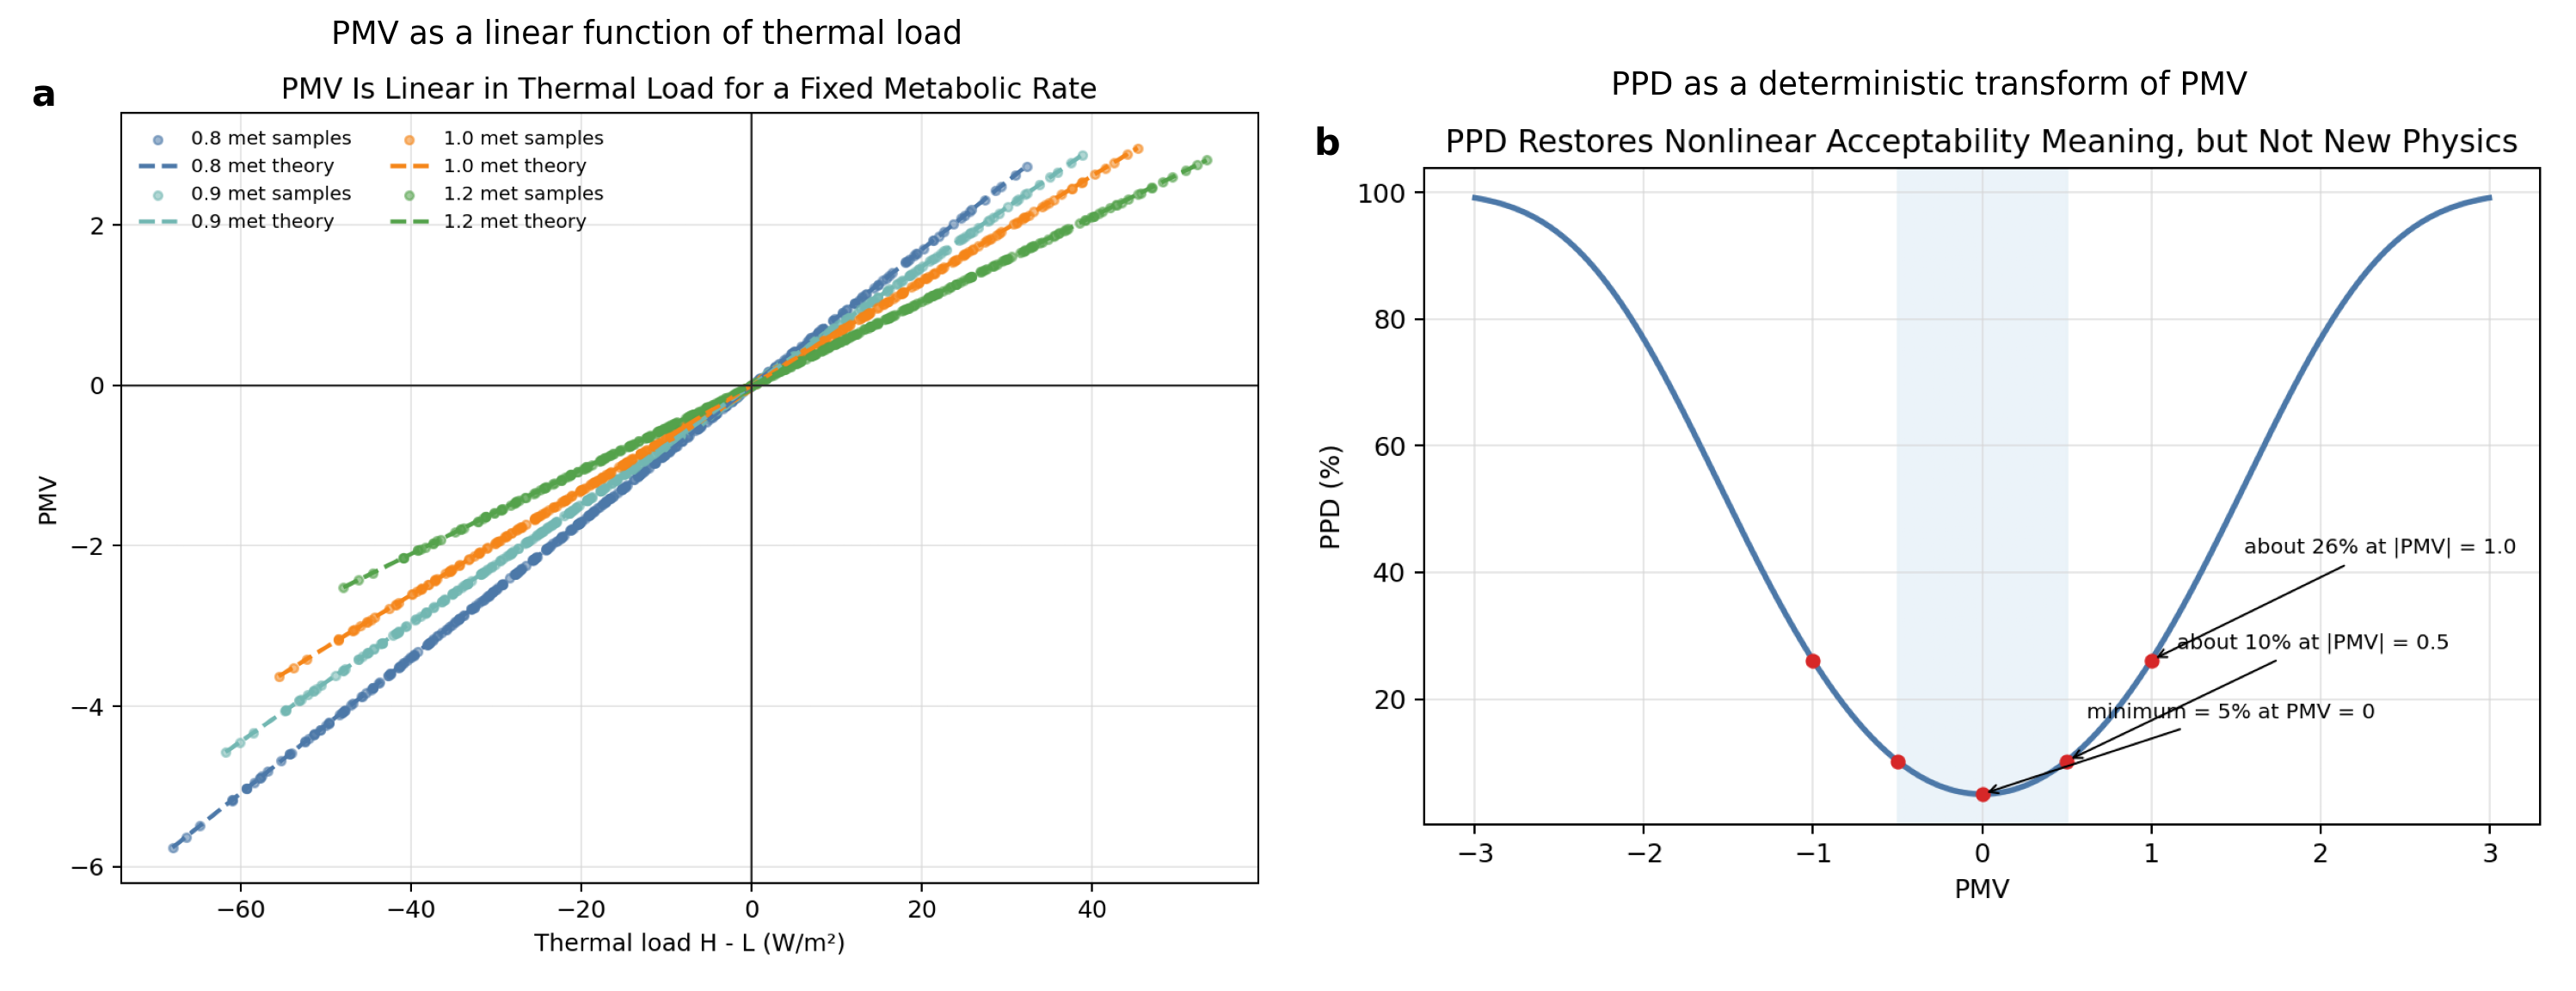
\includegraphics[width=\textwidth]{fig01_pmv_foundations.png}
\caption{Foundations of the PMV critique. (a) PMV is linear in thermal load for fixed metabolic rate. (b) PPD is a deterministic transform of PMV that restores nonlinear acceptability meaning near neutrality, but not an accuracy metric or additional physical model.}
\label{fig:foundations}
\end{figure}

The neutral point is also not unique. Figure~\ref{fig:zeromanifold} shows that PMV = 0 is a manifold in $(T_a, T_r)$ space rather than a single environmental state. Air temperature and radiant temperature trade against each other along the neutral contour, and the contour shifts further when humidity or air speed changes. This is the first reason PMV becomes a weak sole control target: a single PMV target can correspond to multiple physically distinct indoor states.

\begin{figure}[H]
\centering
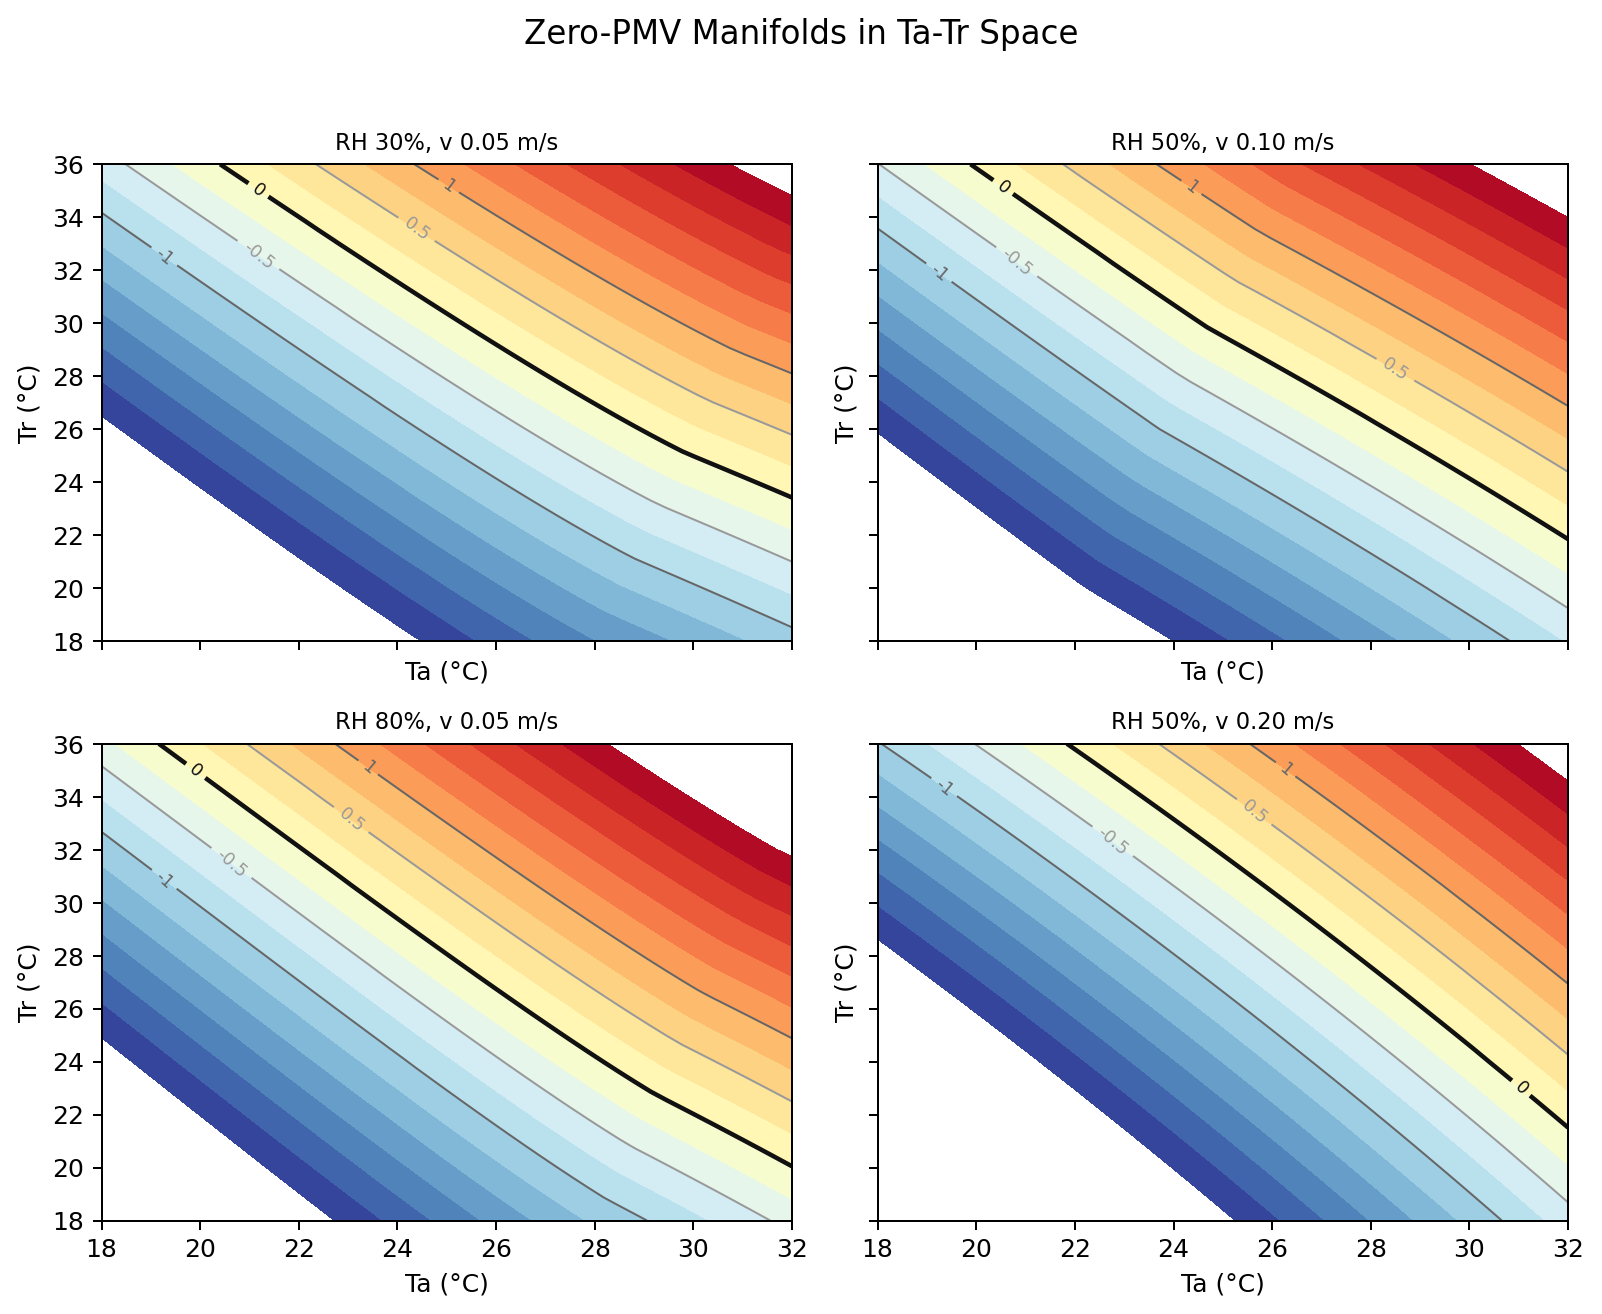
\includegraphics[width=0.9\textwidth]{fig02_zero_manifold.png}
\caption{Zero-PMV manifolds for the reference office occupant under several humidity and air-speed conditions. PMV = 0 is a set of possible states, not a unique thermal environment.}
\label{fig:zeromanifold}
\end{figure}

\subsection{Equal PMV steps imply equal load steps, but not equal control steps}

Figure~\ref{fig:stepresponse} makes the strongest mathematical result explicit. For each fixed profile, the change in occupant thermal load associated with a one-label PMV transition is nearly constant. The one-step thermal-load requirement spans \SIrange{\OneStepLoadMin}{\OneStepLoadMax}{W/person} across the four profiles, but within each profile it remains effectively flat across the tested environmental families. This is a direct consequence of the PMV equation.

The required air-temperature move is not flat. For the reference office profile, moving one label toward neutrality requires between \SI{\ReferenceDeltaTaMin}{\celsius} and \SI{\ReferenceDeltaTaMax}{\celsius}, depending on the starting state. For the larger, more highly clothed profile, the corresponding range widens to \SIrange{\LargerDeltaTaMin}{\LargerDeltaTaMax}{\celsius}. The dissatisfaction meaning is not flat either. Across the tested transitions, one-label PMV recovery changes PPD by \numrange{\OneStepPPDMin}{\OneStepPPDMax} percentage points. The difference between $-3 \rightarrow -2$ and $-1 \rightarrow 0$ is therefore not in the PMV-to-load algebra; it is in the environmental move needed to produce the same PMV step and in the dissatisfaction penalty attached to that step.

\begin{figure}[H]
\centering
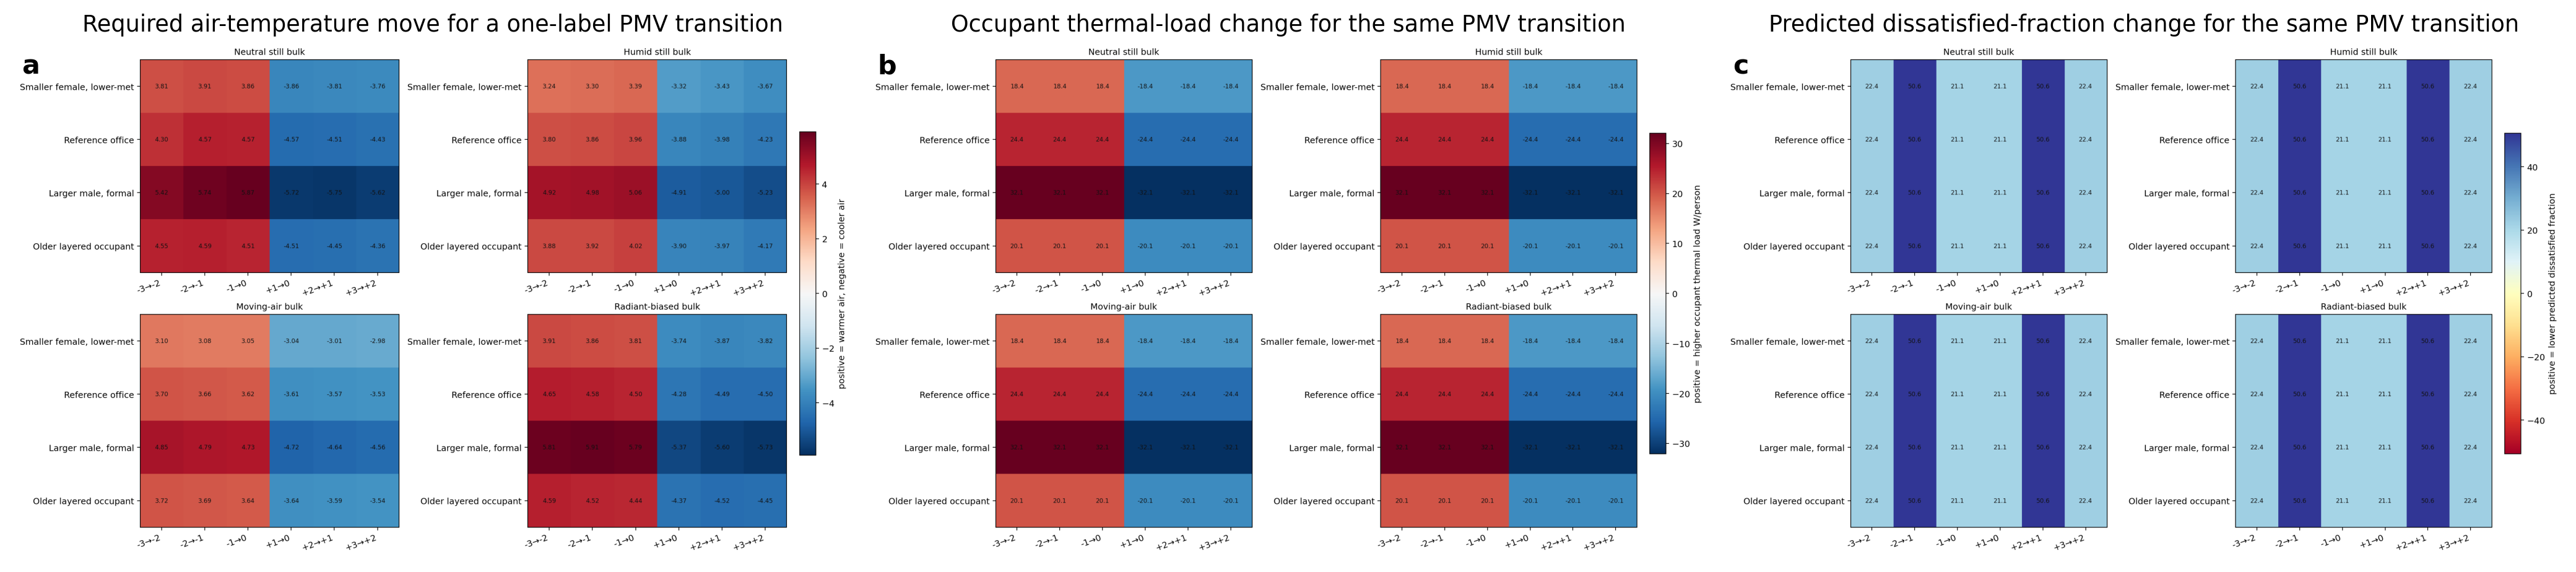
\includegraphics[width=\textwidth]{fig03_step_response.png}
\caption{One-label PMV transitions across occupant profiles and environmental families. (a) The required air-temperature move is not constant across starting states. (b) The corresponding load step remains nearly constant within each profile because PMV is linear in thermal load for fixed metabolic rate. (c) The same one-label PMV step does not produce the same change in dissatisfied fraction because PPD is a nonlinear mapping of PMV.}
\label{fig:stepresponse}
\end{figure}

This result clarifies a key criticism. PMV treats equal changes in mean sensation as equal increments on the scale. PPD partly corrects that by assigning different dissatisfaction changes to those increments, but only after the fact as a scalar remapping. Human meaning and control meaning are still not equal. Borderline and extreme discomfort are separated in the model only by more of the same scalar distance. The model does not distinguish them as qualitatively different control states.

\subsection{Air and radiant moves can have different pathway meanings even when both move PMV toward neutrality}

The directed \SI{1}{\celsius} perturbations show that PMV motion alone is not enough to describe what the system has done. Across the four profiles, directed air shifts improve $|\Delta PMV|$ by \numrange{\AirImproveMin}{\AirImproveMax} on average, whereas directed radiant shifts improve it by \numrange{\RadImproveMin}{\RadImproveMax}. The corresponding mean reduction in dissatisfied fraction spans \numrange{\AirPPDImproveMin}{\AirPPDImproveMax} percentage points for air and \numrange{\RadPPDImproveMin}{\RadPPDImproveMax} percentage points for radiant moves. The air move generally pulls PMV and PPD toward neutrality more strongly in the tested cases, but it does so by moving different pathway watts than the radiant move.

Figure~\ref{fig:profiles} shows the mechanism directly. Air shifts primarily change convective heat loss, with smaller secondary changes in radiation and other terms. Radiant shifts primarily change radiative heat loss. Larger bodies do not automatically experience larger PMV changes, because PMV is area-normalized, but they do show larger total watt changes in \si{W/person}. This is the second reason PMV is a weak sole control variable: the same apparent PMV or PPD improvement can arise from different pathway redistributions with different embodied physical meaning.

\begin{figure}[H]
\centering
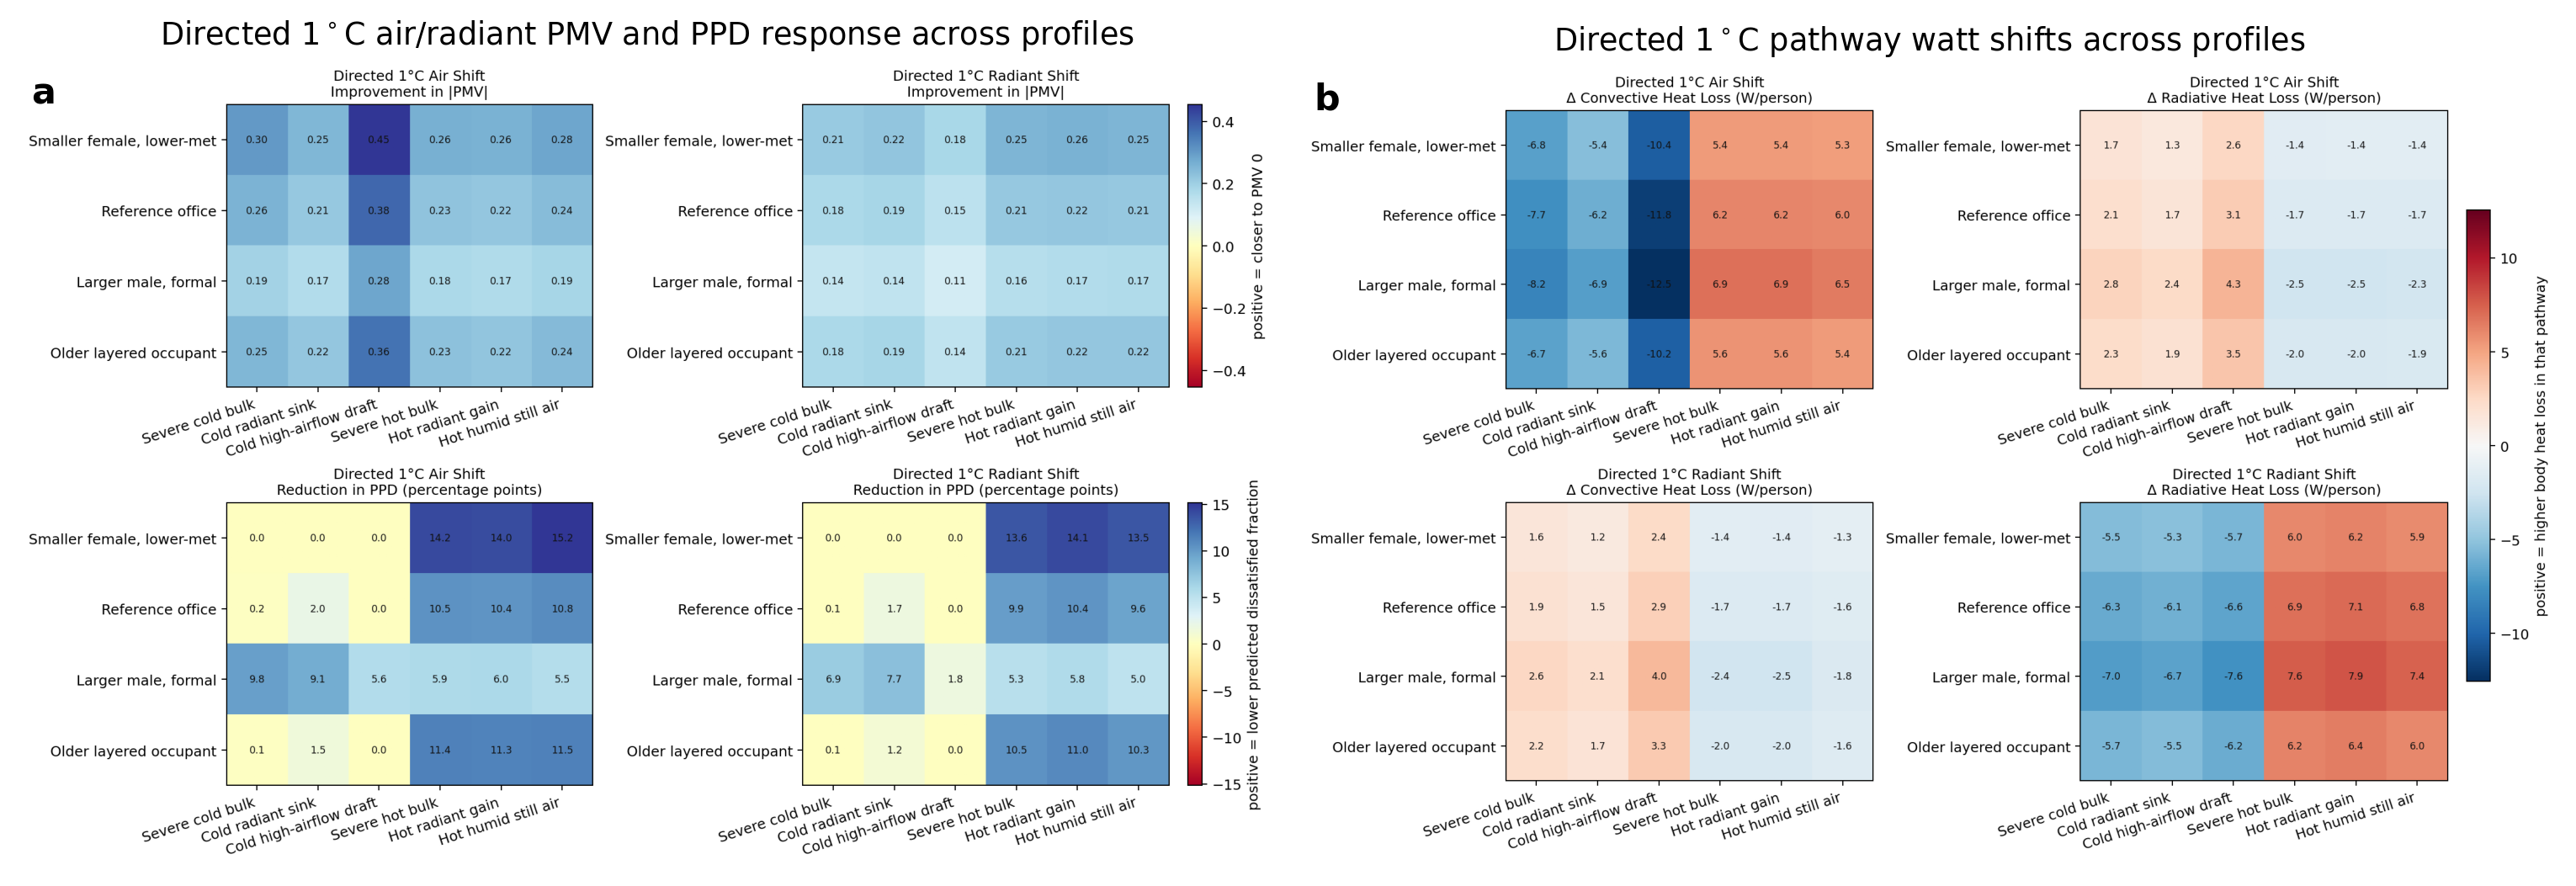
\includegraphics[width=\textwidth]{fig04_profile_pathways.png}
\caption{Profile-sensitive directed \SI{1}{\celsius} perturbations. (a) Air and radiant shifts do not move PMV and PPD by the same amount across profiles and discomfort origins. (b) The same PMV and PPD motion can arise from different convective and radiative watt redistributions.}
\label{fig:profiles}
\end{figure}

\subsection{Recovery ranking changes when system-side exergy is added}

The severe-discomfort study adds a second denominator: system-side exergy. Table~\ref{tab:outcomes} and Figure~\ref{fig:recovery} show the resulting reversal directly. All-air control yields the shortest normalized PMV recovery in \AllAirControlWins/\ScenarioCount\ severe archetypes. However, radiant control minimizes the surrogate system exergy in \RadiantExergyWins/\ScenarioCount.

\begin{table}[t]
\centering
\caption{Air-versus-radiant comparison for the six severe recovery archetypes.}
\label{tab:outcomes}
\begin{adjustbox}{max width=\textwidth}
\begin{tabular}{p{2.5cm}cccccccc}
\toprule
Scenario & Air move & Air PMV & Air exergy & Air dom. & Rad move & Rad PMV & Rad exergy & Rad dom. \\
\midrule
Severe cold bulk & 13.2 & -0.50 & 265.6 & convection & 15.8 & -0.48 & 198.0 & radiation \\
Cold radiant sink & 10.9 & -0.48 & 219.3 & convection & 12.5 & -0.50 & 156.7 & radiation \\
Cold high-airflow draft & 11.0 & -0.49 & 221.3 & convection & — & — & — & — \\
Severe hot bulk & 7.1 & 0.49 & 142.9 & convection & 7.7 & 0.48 & 79.0 & radiation \\
Hot radiant gain & 6.5 & 0.49 & 130.8 & convection & 7.3 & 0.50 & 74.9 & radiation \\
Hot humid still air & 6.4 & 0.48 & 128.8 & convection & 7.6 & 0.49 & 77.9 & radiation \\
\bottomrule
\end{tabular}
\end{adjustbox}
\begin{flushleft}\footnotesize Air and radiant are shown side by side rather than only as winners. The recovery-ranking reversal is meaningful because both levers reach nearly the same recovered PMV in five of the six scenarios, while their estimated exergy requirements differ substantially.\end{flushleft}
\end{table}


This divergence is not a minor accounting detail. Table~\ref{tab:outcomes} makes the point more clearly than a winner summary alone. In \textit{severe cold bulk}, air and radiant both recover to approximately PMV $=-0.5$, but air requires \SI{265.6}{W} of surrogate exergy while radiant requires \SI{198.0}{W}. In \textit{hot radiant gain}, both recover to approximately the same PMV again, yet air requires \SI{85.6}{W} while radiant requires \SI{74.9}{W}. An all-air move can therefore be the fastest route in control space while being the worse route in approximate plant work. PMV does not encode that difference. Once again, the scalar is compressing distinct physical and operational meanings into one target.

\begin{figure}[H]
\centering
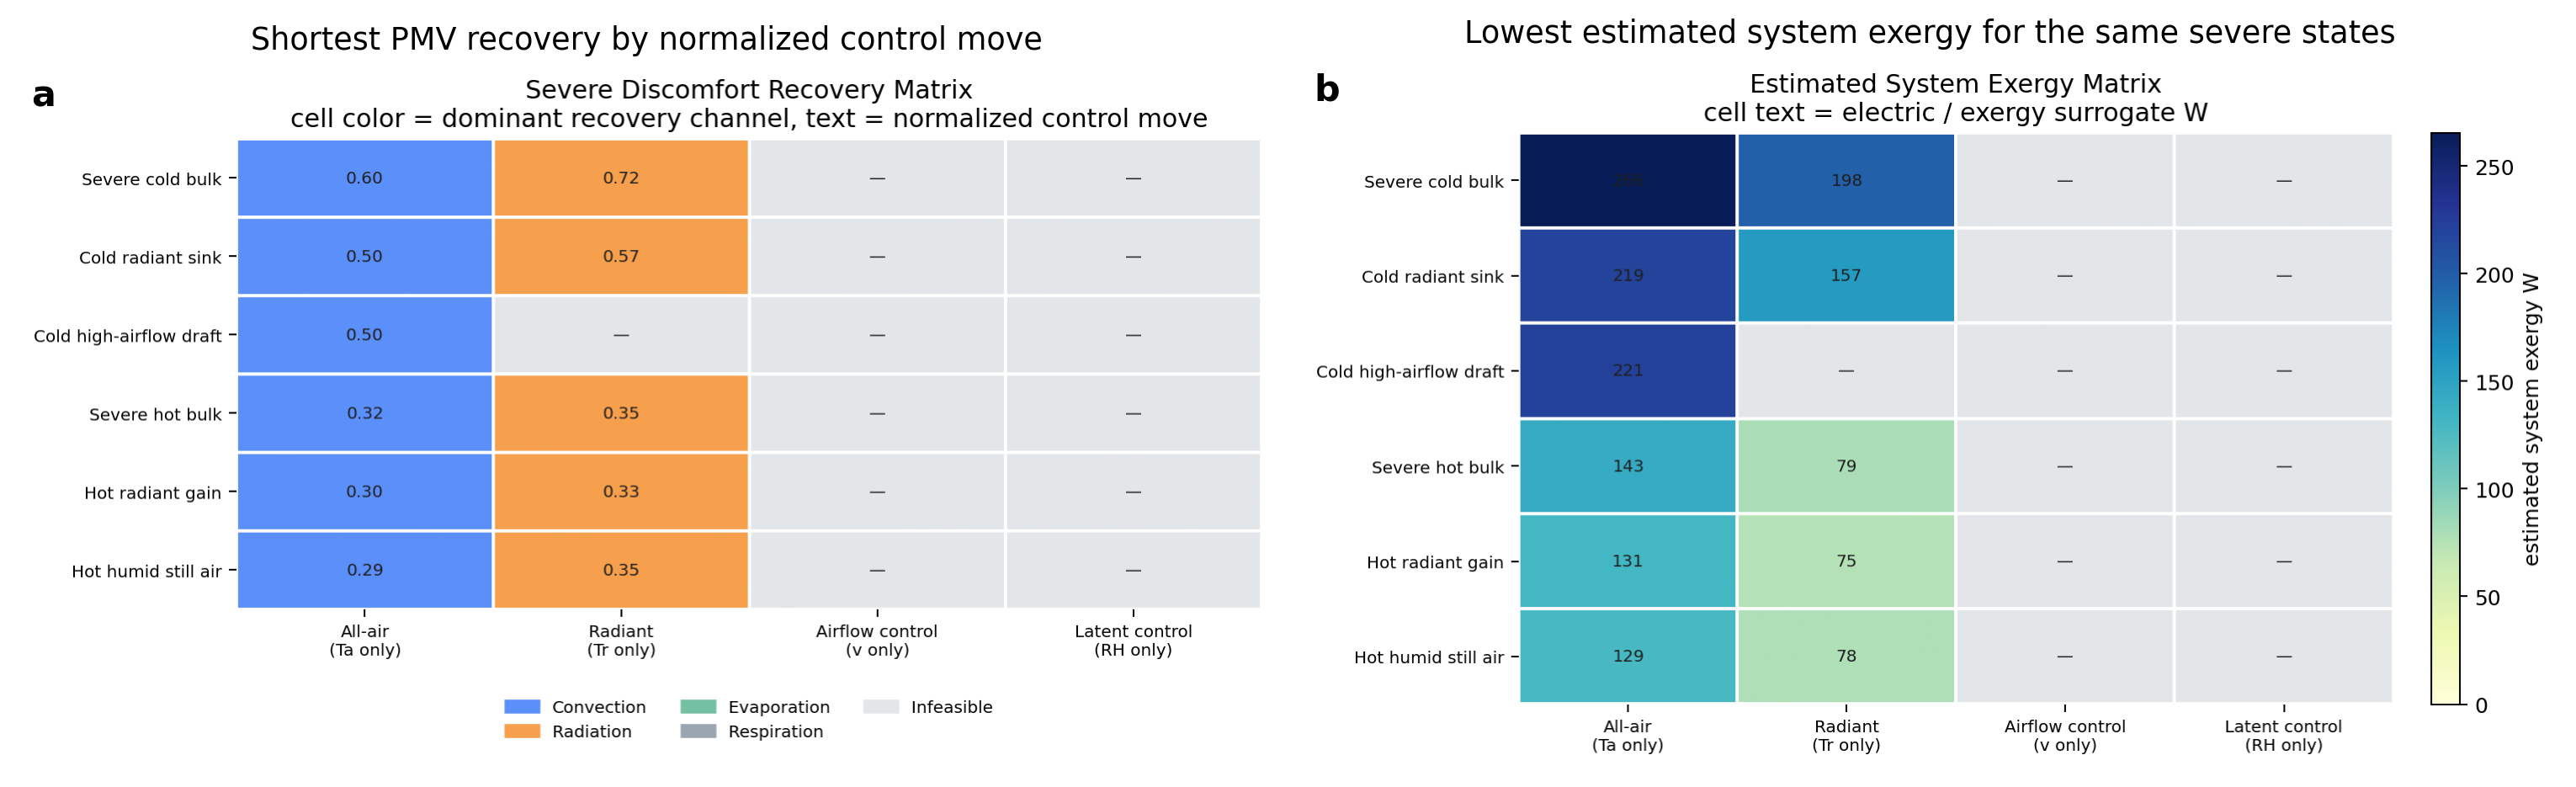
\includegraphics[width=\textwidth]{fig05_recovery_exergy.png}
\caption{Severe discomfort recovery under two denominators. (a) Recovery judged by normalized control displacement favors all-air in all six archetypes. (b) Recovery judged by estimated system exergy favors radiant control in five of the six archetypes.}
\label{fig:recovery}
\end{figure}

\section{Discussion}

The paper does not show that PMV is useless. It shows something narrower and more important: PMV is a bounded steady-state comfort descriptor, but it is a weak sole control variable because it collapses different meanings into one number. PPD partially repairs that collapse at the comfort rim by adding a dissatisfaction penalty, but it does so only by transforming PMV, not by introducing new pathway or physiological knowledge. The model has no difficulty reporting a PMV target. The ambiguity appears when that target is treated as if it already contains pathway meaning, discomfort severity, and system consequence.

This ambiguity operates at three levels. First, PMV is underdetermined with respect to the environment. The same target can be reached by multiple $(T_a, T_r, RH, v)$ combinations. Second, PMV is underdetermined with respect to pathway physics. The same PMV movement can arise from different redistributions of convective and radiative heat loss. Third, PMV is underdetermined with respect to system action. The same recovered PMV can imply different exergy requirements depending on how the control is delivered. The evidentiary consequence is that PMV agreement cannot be treated as physical equivalence.

This is where the pathway framing becomes useful. Convection, radiation, evaporation, and respiration should not be treated here as isolated topics or rival coefficients; they are conditional closures inside the same occupant heat balance. PMV hides those closures once the terms have been summed. That is acceptable if the task is only to report a bounded steady-state comfort index near neutrality. It is inadequate if the task is to interpret why the state changed, which lever owns the correction, or what kind of system action should be preferred.

The profile results sharpen the critique. In the standard PMV formulation, a one-step PMV change corresponds to a fixed thermal-load step within a given profile. Table~\ref{tab:stepsummary} shows why this is not enough. For the reference office profile, the neutral-still transitions all require the same \SI{24.4}{W/person} load change, but $-3 \rightarrow -2$ needs \SI{4.30}{\celsius} while $-2 \rightarrow -1$ and $-1 \rightarrow 0$ need \SI{4.57}{\celsius}. The associated dissatisfaction changes are also different: about 22.4 percentage points for $-3 \rightarrow -2$, 50.6 for $-2 \rightarrow -1$, and 21.1 for $-1 \rightarrow 0$. Equal PMV steps are therefore equal only in the narrow algebraic sense of load; they are not equal in control displacement or acceptability meaning.

PPD adds something useful, but less than it first appears. It does restore a nonlinear interpretation of the comfort rim. This is why the step tables and heatmaps can distinguish the operational meaning of $-2 \rightarrow -1$ from $-1 \rightarrow 0$ even though PMV treats them as equal unit steps. But PPD is still only a scalar transform of PMV. It does not reveal whether the change came through convection or radiation, and it does not distinguish local discomfort from whole-body neutrality. PPD therefore helps interpret acceptability but cannot solve the control problem by itself.

The metabolic-rate update sharpens the same point. Once the reference occupant is moved from a default `1.0 met` office assumption toward `0.9 met`, the PMV factor changes and the one-step load required for recovery changes with it. That is not a secondary sensitivity. It means the apparent precision of PMV-based control is partly an artifact of the occupant normalization embedded in the model. A control signal that already depends on a hidden default body and activity assumption should not be treated as self-sufficient.

The exergy comparison then exposes the control consequence. PMV-based control ranking favors all-air recovery because it is judged by its success in moving a scalar sensation metric. Exergy-aware ranking shows that the same severe states can favor radiant recovery when the denominator becomes system work. Put plainly, PMV-only control is not neutral. It privileges the control variable over the physical and system mechanisms that actually produce comfort. For building operation, the practical implication is straightforward: PMV and PPD remain reasonable reporting and compliance variables near neutrality, but optimization should not stop there. A credible control objective must also preserve pathway meaning, guard against local discomfort, and account for the system cost of delivering the recovery.

\section{Limitations}

The present manuscript is a model-logic study, not a validation study. It does not compare model outputs against measured TSV or physiological data. It also retains several standard PMV simplifications. Clothing enters through insulation and clothing-area factor, not through explicit exposed-skin fraction or body-segment geometry. Body size changes total \si{W/person} pathway quantities but not PMV directly once quantities are normalized by body area. The exergy layer is a surrogate ranking model rather than a full building systems simulation. Finally, the severe-discomfort experiments use one representative office occupant, while the profile-sensitive experiments use four normative archetypes rather than sampled populations.

These limitations bound the claims, but they do not weaken the paper's core argument. The critique is not that PMV fails because this specific implementation is imperfect. The critique is that even under a standard and internally consistent PMV implementation, the scalar itself is insufficient as a sole control objective.

\section{Conclusion}

This paper set out to test whether PMV can carry the meanings often assigned to it in thermal control practice. Under the current ISO 7730 implementation, PMV is linear in thermal load for fixed metabolic rate, PPD is a deterministic dissatisfaction transform, and PMV = 0 is a manifold rather than a unique state. One-label PMV transitions therefore imply fixed load steps within a profile but not fixed air-temperature steps, fixed pathway redistributions, or fixed system effort. Directed \SI{1}{\celsius} air and radiant shifts further show that similar PMV motion can arise from different convective and radiative watt changes. Severe-discomfort recovery finally demonstrates that PMV-based recovery ranking and exergy-based recovery ranking are not the same.

The practical conclusion is straightforward. PMV and PPD remain useful as bounded steady-state comfort indices near neutrality. They should not be treated as sufficient control variables by themselves. PPD improves the interpretation of PMV near the comfort rim, but it does not change the underlying pathway or system ambiguity. Control interpretation therefore requires at least three additional layers: pathway meaning, local discomfort meaning, and system-side cost. Without those layers, PMV-only control mistakes scalar agreement for physical equivalence.

\bibliographystyle{elsarticle-harv}
\bibliography{references}

\end{document}
